% section 1
% Kota Miura (miura@embl.de)

\section{Basics of Basics}

Handling of digital images in scientific research requires knowledge on
the characteristics of digital images. A digital image translates to numbers and is hence a quantitative signal by nature. In this section, we learn the very basics of the numerical nature of digital images. Inappropriate handling not
only lowers the quality of your analysis, but it could also be possible
that your processing is considered as a "manipulation
of data". For this latter point, please also refer to
\citet{Rossner2004}. There are some limits on acceptable image processing
to maintain the scientific validity. Standards on scientific image
processing could be found in "Digital Imaging:
Ethics" by \citet{Cromey2010}. 

\subsection{Digital image is a matrix of numbers}
\label{subsec:imageEQmatrix}
A digital image we display on a computer screen is made up of pixels. We can see
individual pixel by zooming up the image using the magnifying tool\footnote{\
Zooming in / out of the image does not change the content of the image.}. Width
and height of the image are defined by the number of pixels in x and y
directions. Each pixel has brightness, or intensity (or more strictly,
amplitude) somewhere between black and white represented as a number. Within
an image file saved in a computer hard disk, the intensity value of each pixel is written. The value is converted to the grayness of that pixel on monitor screen.
We usually do not see these values, or numbers, in the image displayed on
monitor, but we could access these numbers in the image file by converting 
the image file to a text file \footnote{It's also possible in a limited way by
moving the mouse pointer over the image and checking the number indicated in
ImageJ menu bar.}.

\begin{indentexercise}{1}
\label{exer:1111}
\item Conversion of image to a text file
\item Make a new image by \ijmenu{[File > New > Image\ldots]}. In dialog window,
make a new image with the following parameters:

\begin{itemize}
\item name = test.txt
\item type = 8bit
\item Fill with Black
\item 10 pixel width
\item 15 pixel height
\item Slices = 1
\end{itemize}


%figure
\begin{figure}[htbp]
\begin{center}
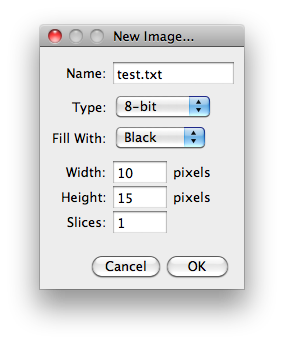
\includegraphics[width=5cm]{fig/CMCIBasicCourse201102-img1.png}
\caption{ New Image Dialog}
\label{fig:img1}
\end{center}
\end{figure}
Clicking "OK", you will see a new window showing a black image (Fig.
\ref{fig:mostbasic}). At the top of the window you can see the file dimension ("10 x 15"), 
bit-depth and the file size (I will explain these values later.
). Take the pen tool and draw some shape (what ever you want. 
If you do not see anything drawn, then you need to change the color of the pen to white by 
\ijmenu{[Edit > Option > Colors\ldots]} and set Foreground Color to white). 
Then do \ijmenu{[File > Save as > Text image]} and save the file. \\

You will find that the name of the file ends with ".txt". 
Open File Explorer (Win) or Finder (Mac) and double click the file. 
The file will be opened in text editor.

What you see now in the text editor is a "text image", a 2D
matrix of tab-delimited numbers. At the left most column in the example
(Fig. \ref{fig:mostbasic2}), there are only zeros. This corresponds to the left column
pixels in the image, where the color is black. In the middle in the
example image, there are several "255".
These are the white part of the image.
In the text image, edit one of the numbers (either 0 or 255) and change
to 100. Then save the file with a different name, such as
"temp.txt". Then in ImageJ open the file by \ijmenu{[File > Import > Text
Image\dots]}. You should see some difference in the image now. 
The image now has a dark gray dot, not black nor white.
\end{indentexercise}

%double figure
\begin{figure}[htbp]
\centering
\subfloat[]{\label{fig:img2}
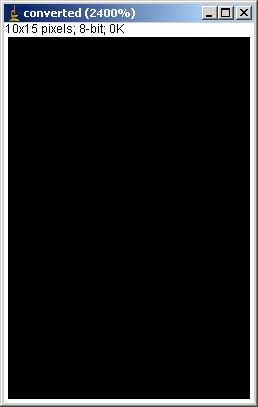
\includegraphics[width=3cm]{fig/CMCIBasicCourse201102-img2.jpg}
}
\subfloat[]{\label{fig:img3}
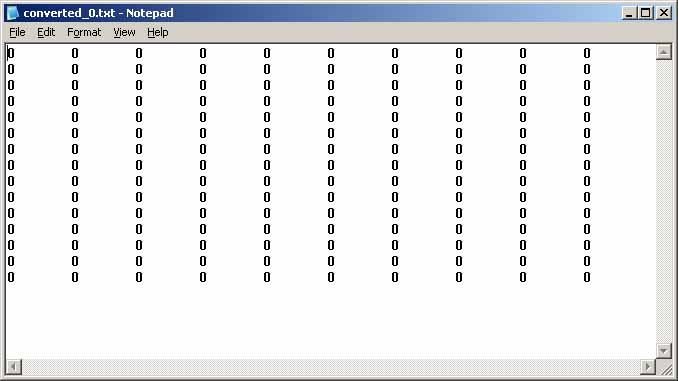
\includegraphics[width=9cm]{fig/CMCIBasicCourse201102-img3.jpg}
}
\caption{ A digital image (b) is a matrix of numbers (b).}
\label{fig:mostbasic}
\end{figure} 

%double figure
\begin{figure}[htbp]
\centering
\subfloat[]{\label{fig:img4}
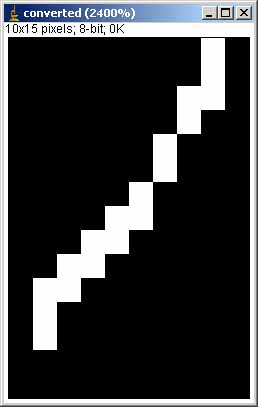
\includegraphics[width=3cm]{fig/CMCIBasicCourse201102-img4.jpg}
}
\subfloat[]{\label{fig:img5}
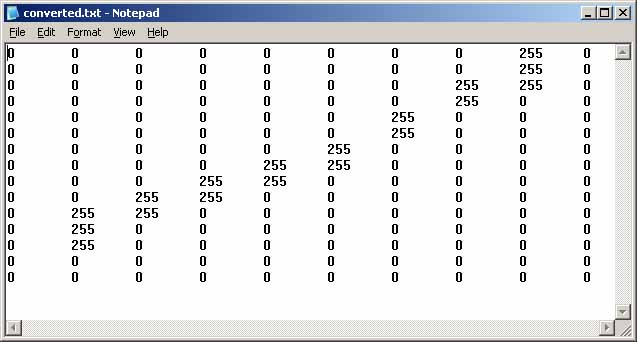
\includegraphics[width=9cm]{fig/CMCIBasicCourse201102-img5.jpg}
}
\caption{ White line (a) corresponds to non-zero numbers (b).}
\label{fig:mostbasic2}
\end{figure} 


Note: The pixel values are not written to the hard disk as a 2D matrix but as
a single array. The matrix is only reproduced upon loading according to the width
and height of the image. Pixel values of image stacks (3D or 4D), are
also in 1D array in hard disk. 3D or 4D matrix is reproduced according
to additional information such as slice and channel number. Such
information is written in the
"header" region of the file, which
precedes the "data" region of the
file where the 1D array of pixel array is contained. The header structure
 depends on the file format, many such formats exist (the most common are TIFF or BMP, we will
see more in "file formats and
header" section). 



\subsection{Image Bit-Depth}
\label{subsec:bitdepth}
Image file has a defined bit depth. You might have already
heard terms like "8-bit" or
"16-bit" and these are the bit depth. 8-bit
means that the gray-scale of the image has $2^{8} = 256$
steps: in other words, the grayness between black and white is divided
into 256 steps. In the same way 16-bit translates to $2^{16} = 65536$ steps, hence for 16-bit images one can assign gray-level to pixels in a much more
precise way; in other words "grayness
resolution" is higher. 

\begin{quote}
Microscope images are generated
mostly by CCD camera (or something similar). 
CCD chip has a matrix of sensors. Each sensor receives
photons and converts the number of photons to a value for a
pixel at the corresponding position within the image. Larger bit-depth
enables more detailed conversion of signal intensity (infinite steps) to pixel values (limited steps).
\end{quote}
Why do we use "$2^{n}$"? This
is because computers code the information with binary numbers. In binary the elementary units are called bits and the only possible values are 0 and 1 (in the decimal system these units are called digits and can take values from 0 to 9).
Coding values with 8-bit means for example that this value is represented as an 8 bit number, something like "$00001010$" ( $= 10$ in
decimal). Then the minimum value is =
"$00000000$" ("0" in decimal) and the maximum is $11111111$
("255" in decimal). 8-bit image allows 256
scales for the grayness (using calculator application in your computer,
you could easily convert binary number into normal decimals and vice
versa). In case of 16-bit image, the scale is $2^{16}$ so
there are 65536 steps. 


We must not forget that the nature is continuous. In conventional
mathematics (as you learn in school), a decimal point enables you to represent
infinite steps between 0 and 1. But by digitizing the nature we lose
the ability to encode infinite steps such that 0.44 might be rounded to 0 and 0.56 to
1. Thus, the bit-depth limits the resolution of the analog to digital
conversion (AD conversion). Higher bit depth generally allows higher
resolution.\\
\\
ImageJ has a high-bit-depth format called signed 32-bit floating point
image. In all above cases with 8-bit and 16-bit, the pixel value is
represented in integer but floating-point type enables decimal points
(real number) for the pixel value such as
"15.445". Though 32-bit floating point
image can be used for image calculation, many functions in ImageJ do
not handle them properly, so cares should be taken when using this image format. If
you want to know more about the 32-bit format, read the following box
(a bit complicated; you could just pass through):

\begin{quotation}
32 bit FLOATING POINT images utilize efficient use of the 32 bits.
Instead of using 32 bits to describe 4,294,967,296 integer numbers, 23
bits are allocated to a fraction, 8 bits to an exponent, and 1 bit to a
sign, as follows:\\
~\\
$V = (-1)^{}S * 1.F * 2^{}(E-127)$,\\ 
whereby:\\
S = Sign, uses 1 bit and can have 2 possible values\\
F = Fraction, uses 23 bits and can have 8,388,608 possible
values\\
E = Exponent, uses 8 bits and can have 256 possible values\\
~\\
Practically speaking, this allows for an almost infinite number of tones
between level "0" and
"1", more than 8 million tones between
level "1" and
"2" and 128 tones between level
"65,534" and
"65,535", much more in line with our human
vision than a 32 bit integer image. Because of the infinitesimally
small numbers that can be stored, the 32 bit floating point format
allows to store a virtually unlimited dynamic range. In other words, 32
bit floating point images can store a virtually unlimited dynamic range
in a relatively compact way with more detail in the shadows than in the
highlights and take up only twice the size of 16 bits per channel
images, saving memory and processing power. A higher accuracy format
allows for smoother dynamic and tonal range compression.\\
\\
(Quote from \url{http://www.dpreview.com/learn/?/key=bits})
\end{quotation}

\subsubsection{Guide Line for the Choice of Bit-Depth}

In fluorescence microscopy, the choice of whether to use higher bit-depth format depends on a balance among the intensity of excitation light,  the emision signal intensity, the sensitivity of photon detector, quantum efficiency\footnote{Quantum effeciency is a measure of proportion of photons converted to electric impluse. For example, QE of photographic film is ca. 10\%, that of human eye is 20\%. Recent CCD allows 80\%. } and the gain. If the signal is bright enough then there would good S/N that you could simply use a lower bit depth but if the signal is too bright then you might need to use a higher bit depth just to avoid saturating the bits. This balancing could also be controlled by changing the gain of the camera. In the end, the choice of bit depth depends on what type of measurement you want to achieve. 
If you only need to determine the shape of the target object (``segmentation''), you might not need a higher bit depth image as you could try to adjust the imaging condition rather than increasing the file size of the image. 
On the other hand, if you are trying to measure protein density, a higher bit depth allows you to have more precise measurements so a larger bit-depth is recommended. A draw back is that it takes longer time for data transferring as the bit-depth becomes larger. This may in turn limits the time resolution of image sequences.
The balancing between imaging conditions and the type of  analysis afterward is very much coupled and should be thought well before your experiment. More details on this discussion could be found in microscopy textbook such as \cite{Pawley2006}. 

The choice of bit depth depends on deals with noise. Here is an explanation from S\'{e}bastien Tosi:
\begin{quote}
When minute details need to be preserved in both high and low intensity regions of a sample a large bit-depth is necessary to ensure a good image quality. Indeed for low bit-depth if the signal level is adjusted to avoid saturation in the brightest regions there is a high risk to end up coding the signal of the faintest regions over only very few bits, which has a very detrimental effect on the image quality. A large bit depth is hence necessary to provide a fine slicing of the intensity range while provisioning a sufficient headroom to avoid saturation and as such always the safest option. 

It can be mathematically derived that quantizing a continuous signal to a finite number of levels induces an Additive White (un-correlated) noise commonly called ``quantization noise''. The level of this noise source is conditioned by the number of levels that are allowed (over the effective range of the signal). Depending on the image intrinsic noise (shot noise at a given photon regime) and the noises coming from the detector and the amplifier electronics this noise can eventually be neglected. One should always make sure that this noise source can be neglected to avoid trashing valuable (available) information.

(personal communication, S\'{e}bastien Tosi)
\end{quote}


\subsection{Converting the bit-depth of an image}

In many occasions, you might want to decrease the bit-depth of image
simply to reduce the file size (16-bit file becomes half the file size
when it is converted to 8-bit), or you might need to use certain
algorithm that is available only with 8-bit images (there are many such
cases), or so on. In any case, this will be a good experience for you
to see the limitation of bit-depth.

Here, we focus on the conversion of a 16-bit image to an 8-bit image to
study its effect and associated possible errors. 


\begin{indentexercise}{1}
Let's first open a 16-bit image from the sample. 
If you have the course plugin installed, choose the menu item \ijmenu{[EMBL > Samples > m51.tif]}. Otherwise, if you have sample images saved in your local machine, open the image by \ijmenu{[File > Open > m51.tif]}. Choose the line selection tool and draw a vertical line 
(should be yellow by default: called line ROI). Then do \ijmenu{[Analyze > Plot Profile\ldots]}. 
A window pops up. See figures \ref{fig:img6} and \ref{fig:img7}.

\begin{figure}[htbp]
\begin{center}
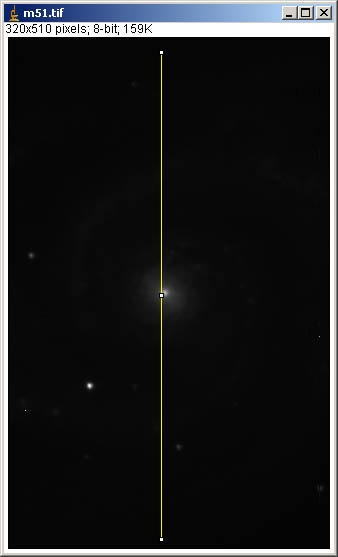
\includegraphics[width=5cm]{fig/CMCIBasicCourse201102-img6.jpg}
\caption{Setting a vertical line Roi.}
\label{fig:img6}
\end{center}
\end{figure}

\begin{figure}[htbp]
\begin{center}
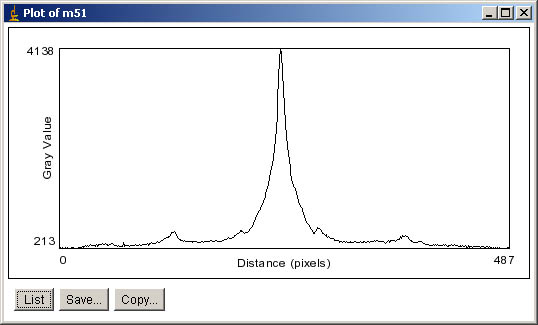
\includegraphics[width=5.694cm,height=3.44cm]{fig/CMCIBasicCourse201102-img7.jpg}
\caption{profile of that ROI}
\label{fig:img7}
\end{center}
\end{figure}

Figure \ref{fig:img6} is the profile of the pixel values along the line ROI 
you just have marked on the image (Fig. \ref{fig:img7}). X-axis is the distance 
from the starting point (in pixel) and the y axis is the pixel value along the line ROI. 
The peak corresponds to the bright spot at the center of the image. 

Let's convert the image to 8-bit. First check the state
of "Conversion" option by
\ijmenu{[Edit > Option > Conversion]}. Make
sure to tick "scale when
converting". 



Do \ijmenu{[Image > Type > 8-bit]}. The line
ROI is still there after the conversion. Do \ijmenu{[Analyze > Plot Profile\ldots] }again. 
You will find another graph pops up. Compare the previous profile (16-bit) and the new profile (8-bit).

Conversion modifies the y-value. Shapes of the profile look
mostly similar, so if you normalize two images, the curve may overlap.
This is because the image is scaled according to the following
formula.

\[
I_{8}(x,y) = \frac{I_{16}(x, y) - min(I_{16}(x,y))}{ max(I_{16}(x,y)) -  min(I_{16}(x,y))} *255
\]

where

$I_{16}(x, y)$: 16-bit image\\
$min(I_{16}(x,y))$: the minimum value of 16-bit image\\
$max(I_{16}(x,y))$: the maximum value of 16-bit image\\
$I_{8}(x, y)$: 8-bit image\\


Save the line ROI you created by pressing "t" or clicking on "add" in the ROI manager (you can open the manager with \ijmenu{[Analyze Tools
ROI manager\ldots]}). A small dialog window pops up, so
click "Add" button in the right side.
The numbers in the left column are names of the ROIs
you add to the manager (they correspond to the coordinates of the start / end points of the ROI).

\begin{figure}[htbp]
\begin{center}
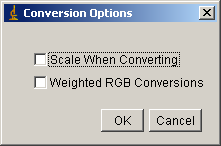
\includegraphics[width=5.847cm,height=3.863cm]{fig/CMCIBasicCourse201102-img8.png}
\caption{Conversion Option. Scaling is turned off in this case. }
\label{fig:img8}
\end{center}
\end{figure}

Now, change the option in \ijmenu{[Edit > Option >
Conversion]} by un-ticking "scale when
converting". Open the 16-bit image again by
\ijmenu{[File > Open > m51.tif]}. Then
again, do \ijmenu{[Image > Type > 8-bit]}.
An apparent difference you can observe is that now the picture looks like a
overexposed image. Find the ROI manager window and click the ROI number
you stored in above. Same line ROI will appear in the new window. Then
do \ijmenu{[Analyze > Plot Profile\ldots]}. This third profile
has a very different shape compared to the previous ones. This is because
the values above 255 are now considered as
"saturated", which means that what ever the
value is, numbers larger than 255 becomes 255.

%figure
\begin{figure}[H]
\begin{center}
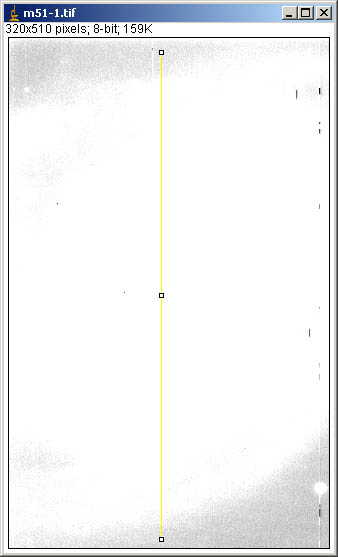
\includegraphics[width=5cm]{fig/CMCIBasicCourse201102-img9.jpg}
\caption{ m51 image converted to 8-bit without scaling.}
\label{fig:img9}
\end{center}
\end{figure}

%double figure
\begin{figure}[H]
\centering
\subfloat[]{\label{fig:img10}
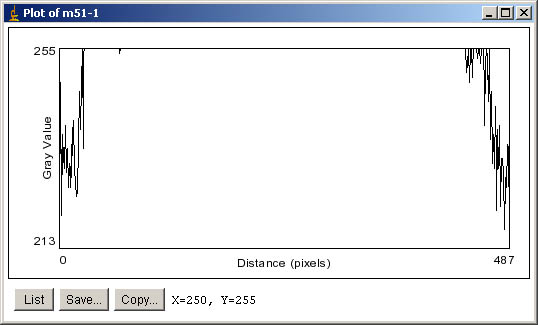
\includegraphics[width=5cm]{fig/CMCIBasicCourse201102-img10.jpg}
}
\subfloat[]{\label{fig:img11}
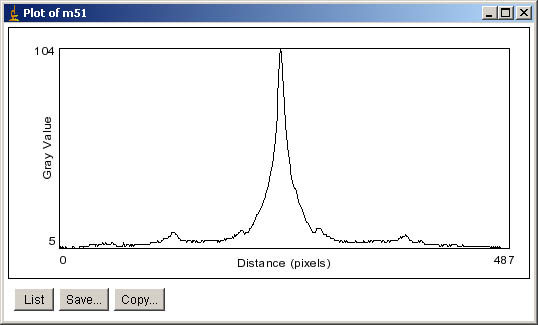
\includegraphics[width=5cm]{fig/CMCIBasicCourse201102-img11.jpg}
}
\caption{ (a) Intensity profile of \ref{fig:img5}. If the conversion is done with scaling, then the profile would look like (b). }
\label{fig:8bitConverted}
\end{figure} 

\end{indentexercise}

When you perform a conversion, very different results could appear depending on
how you scale, like we have just seen. But in many cases, you do not
recognize such changes just by looking at the image: for this reason,
one should keep in mind that the conversion may
"saturate" or cause artifacts in the image
- screwing up scientific images to non-scientific ones. 


\subsection{Math functions}

A digital image is a matrix of numbers. We can calculate images like usual
math. If there is a flat image with pixel value of 10, and if you add 1
to the image, then all pixel values become 11. We think about a pixel
at $(5, 10)$, and we write down the calculation as follows:

\begin{equation}
f(5, 10) = 10
\end{equation}

\begin{equation}
g(5,10) = f (5, 10) +1 = 11
\end{equation}

We generalize this. x and y are the coordinates within the image.

\begin{equation}
g( x , y ) = f (x, y) + 1
\end{equation}

The original image is $f(x, y)$ and the result after the addition
is $g(x, y)$. 

Likewise images could also be subtracted, multiplied and divided by
number. 

\begin{indentexercise}{1}
Simple math using 8-bit image: Prepare a new
image following the initial part of the exercise \ref{exer:1111}. Now,
bring the mouse pointer over the image and check the
"value" that appears in the
status bar in the ImageJ window\footnote{\ In the previous exercise \ref{exer:1111}, 
we converted the image to a text file and then checked the pixel
values, but it is also possible to check the value pixel by pixel using
this method. From ImageJ 1.46i (release: Mar. 15, 2012), 
you could check the pixel values by \ijmenu{[Image > Transform > Image to Results]}. 
This command will send the image matrix shown in Results window as numbers.}. 
All pixel values in the image should be"value = 0".
"x=\ldots, y=\ldots " in the
status bar. 

Commands for mathematical operations in ImageJ are as follows. 

\ijmenu{[Process > Math > Add\ldots]}\\
\ijmenu{[Process > Math > Subtract\ldots]}\\ 
\ijmenu{[Process > Math > Multiply\ldots]} \\
\ijmenu{[Process > Math > Divide\ldots]}\\

%figure
\begin{figure}[htbp]
\begin{center}
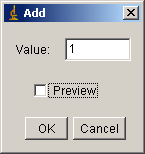
\includegraphics[width=3.8cm]{fig/CMCIBasicCourse201102-img12.png}
\caption{ Add dialog.}
\label{fig:img12}
\end{center}
\end{figure}


Add 10 to the image: Do \ijmenu{[Process > Math > Add{\dots]}}. A dialog window pops up and you can for instance 
input 10 and press OK. Now, place the mouse pointer over the image
to check that the pixel values actually become 10. Then select the pen
tool from the tool bar, and draw a diagonal line in the window. Check
again the pixel value. The line you just drew has pixel value 255. Then
add 10 again to the image by \ijmenu{[Process > Math > Add{\dots]}}. Check the pixels by placing the pointer.
The black part is now 20, but what happened to the white line? 

Since the image bit-depth is 8, the available number is only between 0
and 255. When you add 10 to a pixel with its value 255, the calculation
returns 255 because the number
"265" does not exist in 8-bit
world. A similar limitation applies to other mathematical operations too. If
you multiply a pixel value 100 by 3, the answer in normal mathematics
is 300. But in 8-bit world, that pixel becomes 255. 

How about division? Close the currently working test image, and prepare
a new image as you did in \ref{subsec:imageEQmatrix}. Zoom up the image, and add 100
(\ijmenu{[Process > Math > Add{\dots]}}; you
should see the image turns to gray from black). Check pixel values by
placing the pointer above the image. Now, Divide the image by 3
(\ijmenu{[Process > Math > Divide{\dots]}}).
Check the result by placing the mouse over the image. The pixel value
is now 33. Since there is no decimal placeholder in 8-bit, the division
returns the rounded value of (100 / 3 = 33). One could also divide
image by any real number, such as 3.1415. The answer will be in integer
in all cases in 8-bit and 16-bit. In case of floating point 32-bit
image, the calculation results are different. We study this in the next
exercise. 
\end{indentexercise}

\begin{indentexercise}{2}
Simple Math on 32-bit Image: prepare a new
32-bit image (in the \ijmenu{[New > Image..]} dialog,
select 32-bit from the "type"
drop-down menu). Then add 100 to the image. Check that the image pixel
values are all 100. Then divide the image by 3. Check the answer. This
time the result has a decimal placeholder. 
\end{indentexercise}

Bit-depth limitation of digital image is very important for you to know,
in terms of quantitative measurements. Any measurement must be done
knowing the dynamic range of the detection system prior to the
measurement. \textit{If you are trying to measure the amount of
protein, and if some of the pixels are saturated, then your measurement
is invalid}. 

\subsection{Image Math }

In the previous section we operated on a single image. Likewise, we
can perform computations involving two images. For example, assuming two
images \textit{f} and \textit{g} with same dimensions, and 

\begin{equation}
f(5, 10) = 100
\end{equation}

\begin{equation}
g(5, 10) = 50
\end{equation}

\ldots meaning that the pixel value at the position $(5, 10)$ in the
first image \textit{f} is 100 and in the second image g is 50, we can
add these values and get a new image \textit{h} such that:

\begin{equation}
h(5, 10) = f(5, 10) + g(5, 10) = 100 + 50 = 150
\end{equation}

This holds true for any pixel at position $(x, y)$:

\begin{equation}
h(x, y) = f(x, y) + g(x, y)
\end{equation}

Note that this only works when the image width and height are
identical. Above is an example of addition. More numerical operations
are available in ImageJ: \ 

\begin{center}
\tablehead{}
\begin{supertabular}{|m{4.748cm}|m{6.282cm}|}
\hline
 Add &
 img1 = img1+img2\\\hline
 Subtract &
 img1 = img1-img2\\\hline
 Multiply &
 img1 = img1*img2\\\hline
 Divide &
 img1 = img1/img2\\\hline
 AND &
 img1= img1 AND img2\\\hline
 OR &
 img1 = img1 OR img2\\\hline
 XOR &
 img1 = img1 XOR img2\\\hline
 Min &
 img1 = min(img1,img2)\\\hline
 Max &
 img1 = max(img1,img2)\\\hline
 Average &
 img1 = (img1+img2)/2\\\hline
 Difference &
 img1 =
{\textbar}img1-img2{\textbar}\\\hline
 Copy &
 img1 = img2\\\hline
\end{supertabular}
\end{center}


\begin{figure}[h!]
\begin{center}
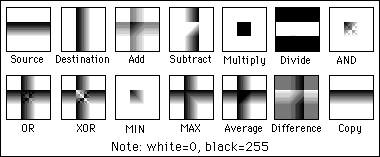
\includegraphics[width=10.945cm,height=4.323cm]{fig/CMCIBasicCourse201102-img13.png}
\caption{Taken from ImageJ web site. \url{http://rsb.info.nih.gov/ij/docs/menus/process.html}}
\label{fig:img13}
\end{center}
\end{figure}

The figure above represents the result of various image math operations. 

\begin{indentexercise}{1}
Image Math -- subtraction:\\
Open Images \textbf{cells\_ActinDNA.tif} and \textbf{cells\_Actin.tif}.
The first image is containing images from two channels. One is actin
labeled, and the other is DNA labeled. We isolate the DNA signal out of
the first image by image subtraction. Do \ijmenu{[Process > Image > Calculator\ldots]}. In the pop-up window, choose the appropriate combination to subtract \textbf{cells\_Actin.tif} from \textbf{cells\_ActinDNA.tif}. Don't forget to tick "Create New Window". 
\end{indentexercise}


\subsection{RGB image}
\label{subsec:rgb}

Color images are in RGB format (could also be a so-called pseudo-color image, or
8-bit color, but this is just because of LUT. See section \ref{subsec:LUT}).
Another popular format is "CMKY" but this
format is optimized for printing purpose (you may have heard it already
when printing something in Photolab). RGB stands for three
primary colors. Red, Green and Blue. If all of them are bright at the
same intensity, then the color is white (or gray). If only red is
bright, then the color is red, and so on. A single RGB image thus has
three different channels. In other words, three layers of different
images are overlaid in a single RGB image. Each channel (layer) has a
bit depth of 8-bit. So a single RGB image is 24-bit image. For this,
the file size of color pics becomes three times larger than a gray scale
8-bit image. Don't save 16bit image in RGB format,
since you lose a lot of information, for automatic conversion from 16
to 8 bit takes place. 

\begin{indentexercise}{1}
Working with RGB image:
 
\item (a) Open the image \textbf{RGB\_cell.tif} by either \ijmenu{[EMBL > Samples]} or \ijmenu{[File > Open]}. Then split the color image to 3 different images \ijmenu{[Image > Color > Split Channels]}. 

\item (b) Merge back the images with \ijmenu{[Image Color > Merge Channels\ldots]}. 

%figure
\begin{figure}[H]
\begin{center}
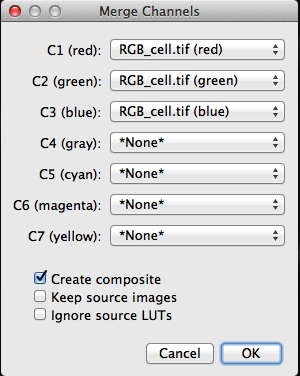
\includegraphics[width=5cm]{fig/dialog_colormerge.png}
\caption{ Color Merge Dialog}
\label{fig:img14}
\end{center}
\end{figure}

In the dialog window, choose an image name for each channel. Uncheck
"Create Composite" and check
"keep source images". Then try
swapping color assignments to see the effect. 

\item (c) Working on each channel separately: Close all windows and
open the "RGB\_cell.tif" again. Do
\ijmenu{[Image > Color > Channel Tools\ldots]}. Then click button "More" and select "Create Composite".
%figure
\begin{figure}[H]
\begin{center}
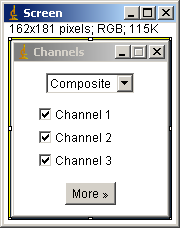
\includegraphics[width=4cm]{fig/CMCIBasicCourse201102-img15.png}
\caption{ Channel Tool}
\label{fig:img15}
\end{center}
\end{figure}

Resulting image is a three-layer stack and each layer corresponds to one
of R, G or B. Each layer can be processed individually. 
%figure
\begin{figure}[H]
\begin{center}
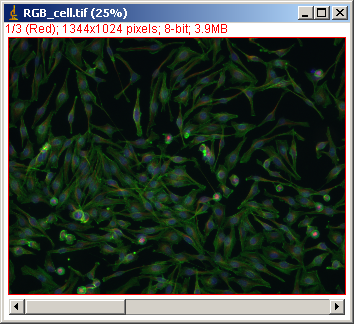
\includegraphics[width=9cm]{fig/CMCIBasicCourse201102-img16.png}
\caption{ Composite image. Note slider at the bottom for switching between three channels.}
\label{fig:img16}
\end{center}
\end{figure}

Using Channel Tools again,
%figure
\begin{figure}[H]
\begin{center}
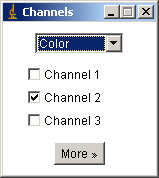
\includegraphics[width=4cm]{fig/CMCIBasicCourse201102-img17.png}
\caption{ Channel Tool, now only selected for Channel 2.}
\label{fig:img17}
\end{center}
\end{figure}

Choose "color" from the pull-down tab, instead of "Composite". Select channel 2 (in this image, this will be Green channel). Select a part of the image using a rectangular ROI. 
%figure
\begin{figure}[H]
\begin{center}
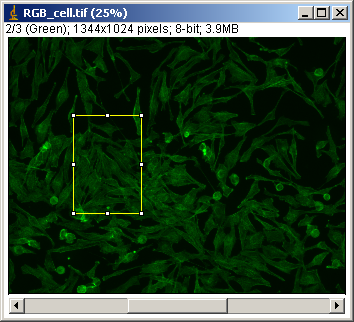
\includegraphics[width=9cm]{fig/CMCIBasicCourse201102-img18.png}
\caption{ ROI selection, in channel 2. Note the position of slider.}
\label{fig:img18}
\end{center}
\end{figure}

Then do \ijmenu{[Edit > Clear]}. This will pop up a window. 
%figure
\begin{figure}[H]
\begin{center}
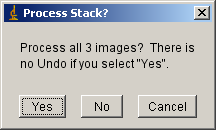
\includegraphics[width=4cm]{fig/CMCIBasicCourse201102-img19.png}
\caption{ Asking you whether you want to process all channels.}
\label{fig:img19}
\end{center}
\end{figure}

Click No, because you want to process only one channel. 
%figure
\begin{figure}[H]
\begin{center}
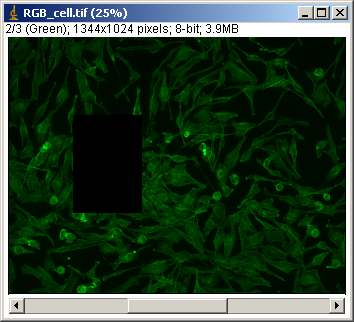
\includegraphics[width=9cm]{fig/CMCIBasicCourse201102-img20.png}
\caption{ Channel 2 pixel values inside selected ROI becomes 0.}
\label{fig:img20}
\end{center}
\end{figure}
\begin{quote}
\textit{Troubleshooting}: If the ROI is not cleared (becomes bright), then you should change the background color setting. Do \ijmenu{[Edit > Option > Colors\dots]} and you will see a pop-up window like this. 
%figure
\begin{figure}[H]
\begin{center}
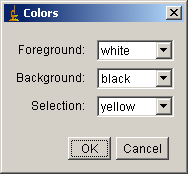
\includegraphics[width=4cm]{fig/CMCIBasicCourse201102-img21.png}
\caption{ Color selection dialog.}
\label{fig:img21}
\end{center}
\end{figure}

Make sure that the background is "black". Do the ROI clearing again. 
\end{quote}
Select "Composite" in the pull-down tab of channel tool. 
%figure
\begin{figure}[H]
\begin{center}
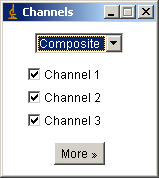
\includegraphics[width=4cm]{fig/CMCIBasicCourse201102-img22.png}
\caption{ Choosing Composite, all channels visual.}
\label{fig:img22}
\end{center}
\end{figure}

Resulting image should look like below. 
%figure
\begin{figure}[H]
\begin{center}
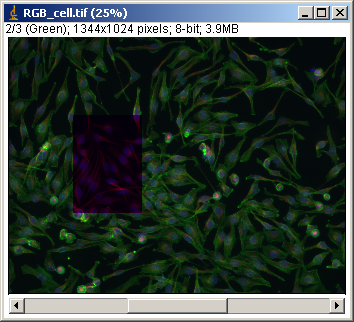
\includegraphics[width=9cm]{fig/CMCIBasicCourse201102-img23.png}
\caption{ Only channel 2 is devoid of image within the selected ROI.}
\label{fig:img23}
\end{center}
\end{figure}

In this case, the intensities of the green channel in the ROI are now set to 0 ("clear"). You could do such
processing of single channel by simply selecting a channel with the horizontal scroll bar and do the processing directly, such as drawing square ROI and deleting that part in that channel in "composite" view. 
\end{indentexercise}

\subsection{Look-Up Table }
\label{subsec:LUT}

We now look at how the matrix of numbers is converted to an image. Let's think about 
a row of pixels with increasing pixel values from 0 to 255 (so there are 256 pixels in this row). 
Computer monitor will show a gradient of intensity that is linearly increasing its brightness 
from black to white. This is because the software is giving a command to the monitor, 
such that "this pixel $(x, y)$ is 158 so the corresponding voltage required for this position $(x, y)$ 
in the screen should be **mV". For this command to be composed, software needs a so called "look-up table" (LUT). 

The default LUT is the gray scale, that assigns black to white from 0 to 255 in the 8-bit image. In the 16-bit image gray scale will be valued from 0 to 65535 between black and white. LUTs are not limited to such grayscales, it could be also colored. We call such colored LUT as ``pseudo-color''. In case of the ``spectrum'' LUT, 0 is red and 100 is green  (see \ref{fig:lutscheme}). The most important point to understand the LUT concept is that with same data, the appearance of the image changes when different LUT is used.  

\begin{figure}[h!]
\begin{center}
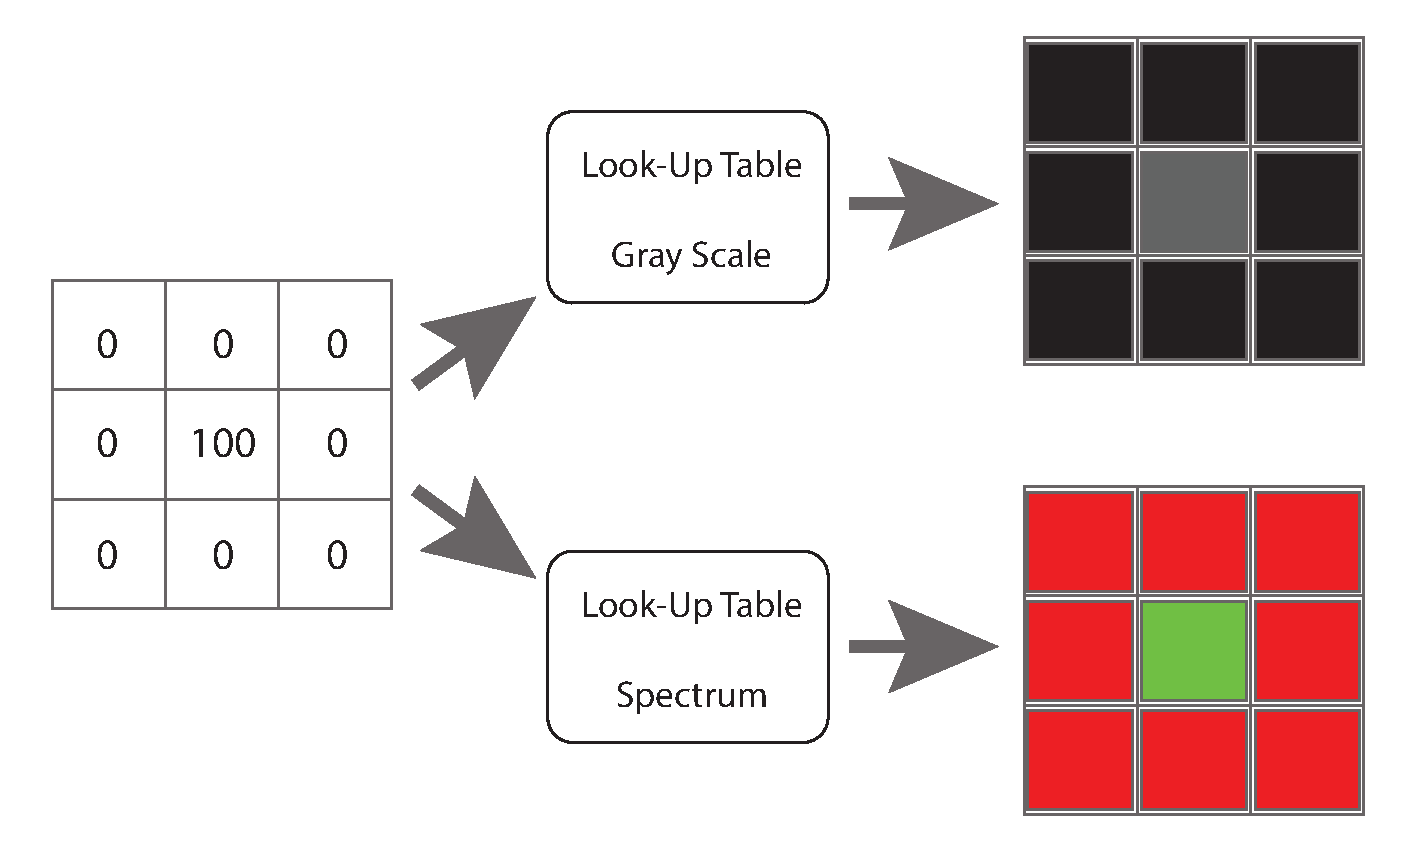
\includegraphics[width=0.9\textwidth]{fig/LUT.pdf}
\caption{Look-Up Table is a table that defines appearance of pixel values as an image. With same pixel values, how they are colored could be different, which depends on the selection of LUT. }
\label{fig:lutscheme}
\end{center}
\end{figure}

This is just like a situation when you start checking a menu in a
restaurant with limited amount of money in your pocket. Say you want to
eat a pizza. You have only \texteuro 10 in your pocket. Looking at the
pizza menu, you will not try to find what you want from names of pizza
and what are the toppings, but instead you will check the prices listed
in the right side of the menu trying to figure out which pizza is less
then \texteuro 10. When you find \texteuro 7.5 in the list, then you slide your
sight to the left side of the menu, and find out that the pizza is
"Margherita". Similar to this,
software first checks the pixel value and then goes to the look-up
table (menu) to find out which brightness should be passed to the
monitor as a command ( = find a convincing price in the menu, then
sliding your sight to the left and find out which pizza to order).





\begin{indentexercise}{1}
For 8-bit images, there is a default LUT normally called "grayscale". 
To see the LUT, open the image \textbf{Cell\_Colony.jpg} and then 
do \ijmenu{[Image > Color > Show LUT]}. LUT window pops up showing 
the relationship between pixel value and pixel intensity. 
Try to change the LUT by \ijmenu{[Image > Lookup Tables >Spectrum]}. 
Pixel value does not change by this operation, but the pixel intensity changes 
that the image appears differently now. Check the LUT again by doing \ijmenu{[Image > Color > Show LUT]}. 
Actual numbers in each LUT could be checked using ``'list' button at the left-bottom corner of each LUT window. 
\end{indentexercise}

%double figure
\begin{figure}[H]
\centering
\subfloat[]{\label{fig:img24}
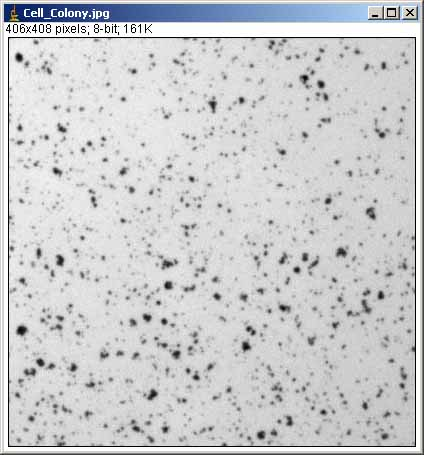
\includegraphics[width=6.371cm,height=6.853cm]{fig/CMCIBasicCourse201102-img24.jpg}
}
\subfloat[]{\label{fig:img25}
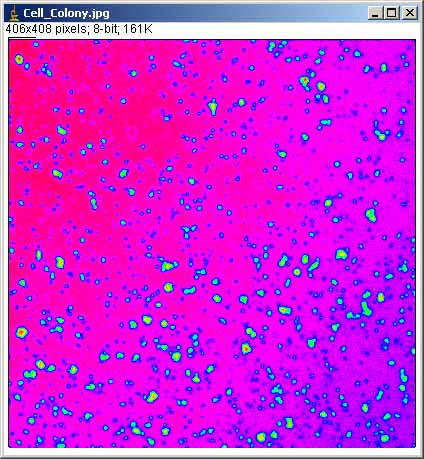
\includegraphics[width=6.431cm,height=6.962cm]{fig/CMCIBasicCourse201102-img25.jpg}
}
\caption{ Grayscale LUT (a) converted to spectrum LUT (b).}
\label{fig:LUTconversionImages}
\end{figure} 

%double figure
\begin{figure}[H]
\centering
\subfloat[]{\label{fig:img26}
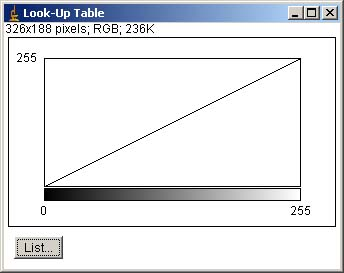
\includegraphics[width=6.055cm,height=4.805cm]{fig/CMCIBasicCourse201102-img26.jpg}
}
\subfloat[]{\label{fig:img27}
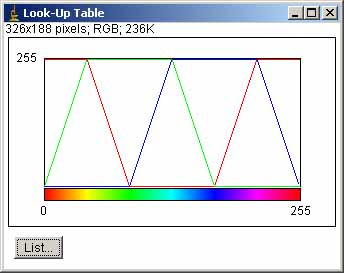
\includegraphics[width=6.103cm,height=4.833cm]{fig/CMCIBasicCourse201102-img27.jpg}
}
\caption{ (a) Grayscale LUT and (b) spectrum LUT}
\label{fig:LUT[lots}
\end{figure} 

\subsection{Image File Formats}

In this part we will discuss on issues related to image file formats including:

\begin{itemize}
    \item Header and Data
    \item Data Compression
\end{itemize}

Image file contains two types of information. 
One is the image data, the matrix of numerical values. 
Another is called "header", which contains the information about the architecture of image. 
Since software must know information such as bit-depth, width and height, and the size of 
the header before opening the image, the information is written in the "header". 
The total file size of an image file is then 

$Total file size = header size + data size$

There are many different types of image formats, such as TIFF, BMP, PICT and so
on. The organization of the information in the header is specific to each format, as is the size of the header. In biology, microscope companies create their own formats to
include more information about the image, such as the type of microscope used,
used objectives, binning, shutter speed, time intervals, user name and so on.

Having to handle company-specific formats makes our life more difficult because each image can a priori
only be opened from the software provided by these companies. Fortunately there
is an excellent ImageJ plugin which enables importing specific image formats to ImageJ
\footnote{\tab LOCI Bioformat Plugin:\\
\url{http://www.loci.wisc.edu/ome/formats.html}}

You do not have to know all the details about the architecture of various image
formats (thanks to the bioformats plugin), but it is important for you to know
that the difference resides mainly in the header. The data part is in most cases
the same, something like what we have seen already using text image (for more
details on header, refer to the appendix \ref{app1} ).

\begin{indentexercise}{1}

\textbf{Accessing the image properties}

Open the example image \textbf{wt1.tif}. Do
\ijmenu{[Image > Show Info\dots]}. Scale (pixels/inch)
is listed in the information window, which was read out from the header
of the image. Then do \ijmenu{[Image > Properties]},
also showing the scale. 
\end{indentexercise}

\textbf{Compression}: Large image files consume a lot of storage space. There are convenient ways to reduce image file size by data compression. When you take a snap shot using a commercial digital camera or a smart phone, the saved image is always compressed.  
But keep in your mind:

There are two types of compression formats: \textbf{loss-less} and \textbf{lossy} formats. In loss-less formats, pixel values generated by CCD are preserved even after the compression is made. On the other hand in lossy formats, pixel values become different from the original measured values and cannot be restored. 

PNG is a popular loss-less compression format that does NOT alter the original pixel values. With this format, compression of images are done by shrinking redundant parts: for example, instead of having 100 pixels of 0 values as a block, you could replace that part by saying ``here, there are 100 pixels of zeros''. If you need to compress files, using PNG format is preferred for scientific image data.  

Other more popular compression formats are like JPEG and GIF. JPEG is ofen used in commercial diginal cameras.  In addition to the redundancy shrinking explained above, the compression procedure tries to mathematically interpolate some parts of the image to ignore small details. These are lossy formats as
the process of compression discards some part of data. This causes artifacts in the image and it could even be "manipulation" of data. For this reason, we better avoid using lossy formats
for measurements as we cannot recover the original uncompressed image once they are converted. 

I recommend not to compress data except for sharing of data for visualization purpose. The PNG format does not lose the original pixel values but due to the file format conversion, the header information associated with the original will be lost and this often causes problem in retrieving important information about images such as scales and time stamps. 

\subsection{Multidimensional data}
\label{sec:stackBasics}

In this section, we study the following topics.

\begin{itemize}
    \item Image stacks
    \item Editing Stacks
    \item 4D stacks
	\item Hyperstacks
\end{itemize}

Multidimensional data, in which we define here as a set of image data with dimensions more than x and y. Multidimensional data have intrinsic limitation in displaying them on two dimensional screen. Efforts have been made to represent multidimensionality in various ways. One way is the ``image stack''.

\subsubsection{stacks}
When you take time-lapse sequence or z-sections using a commercial microscope system, the image files are generally saved in the company specific file formats (\textit{e.g.} .lsm or .lif files). Importing these images into ImageJ could simply be done using LOCI bioformats plugin. 

These image data appear as a series of images contained within a window with a scroll bar at the bottom. By scrolling, one could go through the third dimension like a movie. This is the simplest form of multidimensional representation in 2D display. 

%fig of a stack. 
In some cases, multidimensional data takes a form of multiple
single image frames with numbering such as 


image0001.tif\\
image0002.tif\\
image0003.tif\dots

We can import such numbered files recursively and create a stack in ImageJ. 

\begin{indentexercise}{1}
We import multiple image files as an image stack. Download a zipped file by \ijmenu{[EMBL > Samples > Spindle-Frames.zip]} \footnote{We do also have the stack directly downloadable, but we try to load numberd-tif images here.}. Unzip the file by double clicking. Then
\ijmenu{[File > Import > Image Sequence\ldots]} will open a dialog window and
you must specify the first file of the image series. Select sample sequence
\textbf{eg5\_spindle\_50000.tif\ldots} Then another dialog window pops up (Fig.
\ref{fig:img129}).

%figure
\begin{figure}[H]
\begin{center}
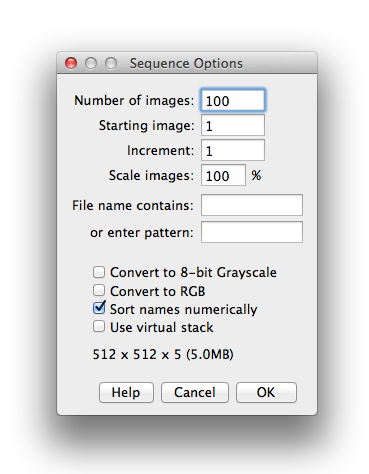
\includegraphics[width=0.7\textwidth]{fig/importSeriesDialog.png}
\caption{ Importing multiple frames as a Stack}
\label{fig:img129}
\end{center}
\end{figure}

ImageJ automatically detects the number of files in the folder, and then another
window opens to ask for the number of images you want to import, the starting image, the increment between the numbering of the files, and also
the common part of the names of the files you want to import.

For example, if your sequence starts with \textit{exp01}\ldots, then you could place the text \textit{exp01} in the text field of ``File name contains''. This then avoids loading other data sets with prefix e.g. \textit{exp02} even if they are within the same folder. Regular expression could also be used in the ``or enter pattern'' text field\footnote{If you do not know what Regular Expression is, try the tutorial at \url{http://www.vogella.com/articles/JavaRegularExpressions/article.html}. For those who knows what regex is, use the Java regex.}. 

There are other options such as scaling and conversion of the image bit depth,
but these operations could be done afterwards. The imported image sequence is within one window, or a stack.

A stack could be saved as a single file. File extension is
typically ".tif", which is same as the single frame file. The file header will contain the
information on the number of frames that the image contains. This number
will be automatically detected when the stack is opened next time\footnote{It is the case in Fiji, but may not be the case for other software.}, so that the stack can be correctly reproduced. 
\end{indentexercise}

Don't close the stack, exercise continues. 

\begin{indentexercise}{2}

In the ImageJ tool bar among all the tool icons, there is a button with ``Stk''. All the commands related to stack can be found there by clicking that icon. 

%figure
\begin{figure}[htbp]
\begin{center}
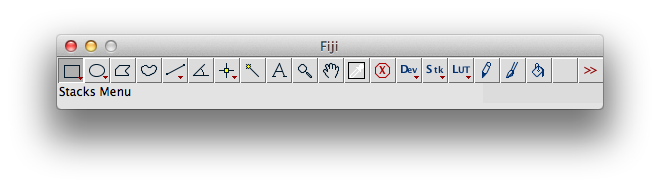
\includegraphics[width=0.9\textwidth]{fig/fijiMenu.png}
\caption{ ImageJ tool bar in default mode.}
\label{fig:img130a}
\end{center}
\end{figure}

\ijmenu{[Start Animation]} plays the sequence as animation. This command can be found at \ijmenu{[Image > Stacks > Tools > Start Animation]}. 
Try changing the playback speed by \ijmenu{[Animation Options]}. This command pops up a dialog to set the playback speed. In the main menu, this same command is at \ijmenu{[Image > Stack > Tools > Animation options\ldots]} 

To exclusively work on stacks, there is an icon >> at the right most position in the ImageJ menu bar. Click and then from drop down menu that appeared, select "Stack tools". Video player-like interface appears in the tool bar (Fig.~\ref{fig:img130b}). Try different buttons to see what actions they perform. 

%figure
\begin{figure}[htbp]
\begin{center}
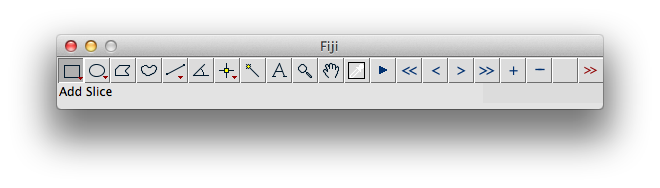
\includegraphics[width=0.9\textwidth]{fig/fijiMenu_StackMode.png}
\caption{ ImageJ tool bar in Stack Tool mode.}
\label{fig:img130b}
\end{center}
\end{figure}

%figure
\begin{figure}[hbtp]
\begin{center}
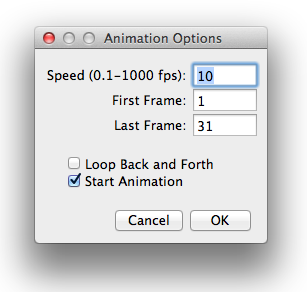
\includegraphics[width=0.6\textwidth]{fig/animationOptions.png}
\caption{ Animation Option Window}
\label{fig:img131}
\end{center}
\end{figure}
\end{indentexercise}

\subsubsection{Editing Stacks}

In many occasions you might need to edit stacks such as
\begin{itemize}
\item Truncate a stack because you only need to analyze a part of the sequence.
\item Combine two different stacks.
\item Add a stack at the end of another stack.
\item Make a combined stack by attaching each frame in a stack by a frame of another stack. Typically, you want to have two channels of image side-by side,
\item Extract every second frame or slices to reduce the stack size by a half. 
\item Split two channel time series to individual time points without splitting the channels. 
\item Insert a small inset within a stack. 
\end{itemize}
For such demands, tools for stack editing are available under the menu tree \ijmenu{[Image > Stack > Tools]}. Fig.~\ref{fig:editStack1} and Fig.~\ref{fig:editStack2a} schematically show what each of these commands does. 
%figure
\begin{figure}[hbtp]
\begin{center}
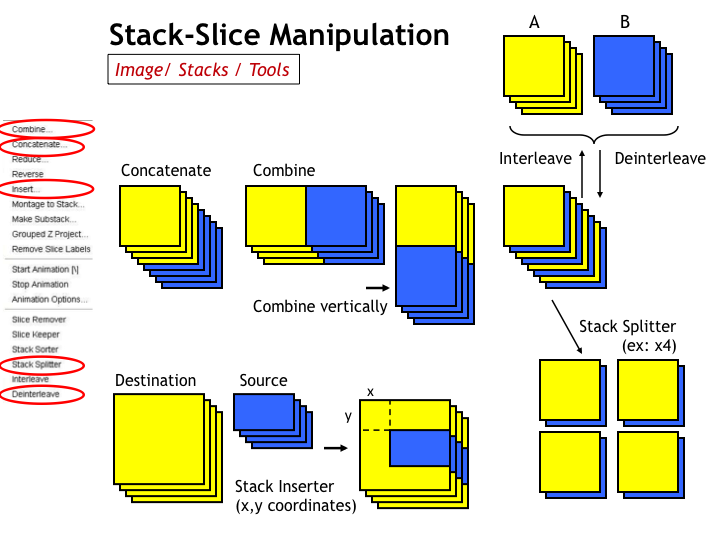
\includegraphics[width=\textwidth]{fig/stackEditing1.png}
\caption{Editing Stacks 1. These commands are under \ijmenu{[Image > Stack > Tools]}. Courtesy of Sebasti\'{e}n Tosi, IRB Barcelona.}
\label{fig:editStack1}
\end{center}
\end{figure}


\begin{figure}[hbtp]
\begin{center}
\includegraphics[width=\textwidth]{fig/stackEditing2.png}
\caption{Editing Stacks 2. These commands are under \ijmenu{[Image > Stack > Tools]}. Courtesy of Sebasti\'{e}n Tosi, IRB Barcelona.}
\label{fig:editStack2a}
\end{center}
\end{figure}


\begin{indentexercise}{1}
\textbf{Creating a Montage}\\
Create a new image \ijmenu{[File > New > Image\ldots]} with the following properties. 
\begin{itemize}
\item Name: could be any thing
\item Type: 8-bit
\item Fill with: Black
\item Width: 200
\item Height: 200
\item Slices: 10
\end{itemize}
Then draw time stamps in each frame by \ijmenu{Image > Stacks > Time Stamper} with the default properties but for the following:
\begin{itemize}
\item X location: 50
\item Y location: 90
\item Font Size: 36
\end{itemize}

Now, you should have printed time for each frame, 0 to 9 sec. To make a montage of this image stack, do \ijmenu{[Image > Stacks > make Montage\ldots]}. Set the following parameters and then click OK. 
\begin{itemize}
\item Columns: 5
\item Rows: 2
\item Border Width: 1
\item Label Slices: checked.
\end{itemize}

\begin{figure}[h!]
\begin{center}
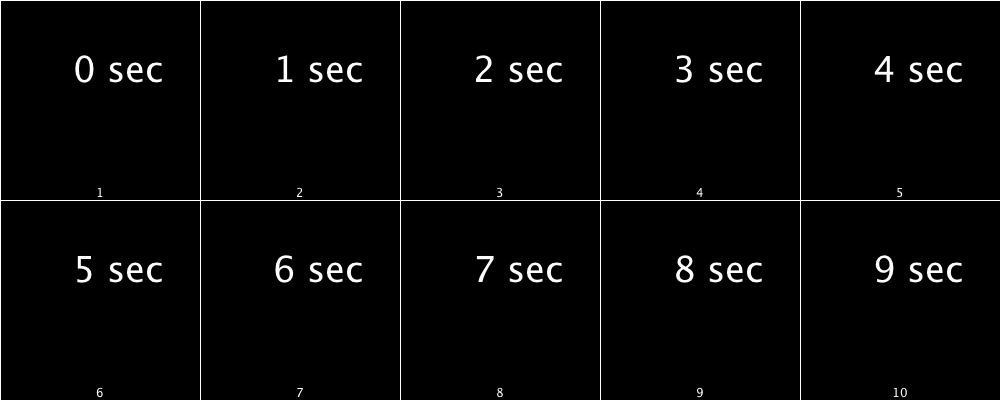
\includegraphics[width=0.8\textwidth]{fig/TimeStampMontage.png}
\caption{Montage of the time-stamped stack.}
\label{fig:editStack2}
\end{center}
\end{figure}

If you have time, try to change the column and row numbers to create montage with different configuration. 

\textbf{Concatenation}

Then duplicate the time stamp stack, concatenate the duplicate to the original (\ijmenu{[Image > Stacks > Tools > Concatenate\ldots]}). Create a montage of this double sized stack. 

\end{indentexercise}


\subsubsection{4D stacks}

A time-lapse sequences (we could call it ``2DT stack'' or xyt stack) or a Z-stack (we could call it ``3D stack'' or xyz stack) are relatively simple objects because they are both made up of a series of two dimensional images. More highly dimensioned data are common these days. In many occasions we take a time series of z-stacks maybe also with multiple channels. The order of two dimensional images within such multidimensional stacks then becomes an important issue. If we take an example of 3D time series, a possible order of 2D images could start first with z-slices and then time series. In this case, the frame sequence will be something like this:

imgZ0-T1.tif\\
imgZ1-T1.tif\\
imgZ2-T1.tif\\
imgZ0-T2.tif\\
imgZ1-T2.tif\\
imgZ2-T2.tif\\
imgZ0-T3.tif\\
\ldots

The number after ``Z'' is the slice number and that after ``T'' is the file name. We often call this order ``XYZT''. Alternatively, 2D images could be ordered with time points first and then z-slices. In this case images will be stacked as:

imgZ0-T1.tif\\
imgZ0-T2.tif\\
\ldots\\
imgZ1-T1.tif\\
imgZ1-T2.tif\\
\ldots\\
imgZ2-T1.tif\\
imgZ2-T2.tif\\
\ldots

We call this order ``XYTZ''. 

The order you will often find is the first one (XYZT) but in some
cases you might also find the second one (XYTZ). 

\subsubsection{Stacks with more than 4D}

If we have multiple channels, we could even have an order like ``XYCZT''\footnote{XYCZT is a typical order but many microscope companies and software do not follow this typical order.} and so on. Since when viewed as a regular stack we can scroll only along a single dimension, the order of stack dimensions is fundamental as it affects the order in which the images will appear. 

To avoid such complication with dimension ordering, there is an advanced format of stack called \textit{Hyperstack}. It can have up to three scroll bars at the bottom for channels (C), slices (Z) and time points (T) so one could easily scroll through the dimension of your choice (Fig.~\ref{fig:heyperstack_mitosis}). 

%figure
\begin{figure}[h!]
\begin{center}
\includegraphics[width=9cm]{fig/Hyperstack_Mitosis.png}
\caption{ A Hyperstack data, showing spindle dynamics. This 5D data could be downloaded by \ijmenu{[File > Open Samples > Mitosis]}}
\label{fig:heyperstack_mitosis}
\end{center}
\end{figure}

We will study more on the actual use of the image stacks in section ``Analysis of Time Series''%\ref{sec:timeseries}.

\begin{indentexercise}{2}
  In this exercise, you will learn how to interact with image stacks (n
  Dimensional images).
  Open sample image stack \textbf{yeastDivision3DT.tif}.
  This is a 3D time series stack. You can browse through the frames by moving
  the scroll bar at the bottom of the frame.
  Since this is a 3D time series, you will see that each time point is a
  sub-stack of images at different optical sections. 
  
  To view the stack in a more
  convenient way, you could convert the stack to a hyperstack by 
  
  \ijmenu{[Image > Hyperstacks > Stack to Hyperstack\dots ]}.\footnote{If this conversion does not work properly, the first thing you could
  check is if the setting of the image dimension is properly set.
  To check this, \ijmenu{[Image > Properties\dots]} and check if slice (z)
  number and frame number (time points) are set correctly.
  For the sample image we use in this exercise, z should be 8 and frames should
  be 46.}
  
   In ``Hyperstack'' mode, two scroll bars appear at the bottom of the
   window. One is for scrolling through z slices and the other to select a time point (frame).
   Each scroll bar could be moved independently of the other dimension, so you
   could for example go through the time series at a same constant z-position,
   or go through z-slices at a certain time point.
   To go back to the normal stack mode, use 
   
   \ijmenu{[Image > Hyperstacks > Hyperstack to Stack\dots]}.
\end{indentexercise}

\subsection{Command Finder}

Commands for these stack related tools (especially editing tools) reside deep inside the menu tree and it is not really convenient to access those commands by manually following the menu tree using mouse. For such a case, and if you could remember the name of the command, a quick way to run the command is to use \textbf{command finder}.

There is a short cut key to start up the command finder: the key ``L''. On start up, the command finder interface looks like figure \ref{fig:commandfinderstart}. Type in the command that you want to use in the text field labeled ``search'', and then the menu items are filtered as you type in (fig. \ref{fig:commandfinderConcat}). Select the one you want and then click the button ``run''. This is the same as selecting that command from the menu tree. This tool is also useful when you know the name of a command but forgot where it is in the menu tree, since it also shows where the command is by showing its menu path. 

\begin{figure}[htbp]
\centering
\subfloat[The interface on start up.]{\label{fig:commandfinderstart}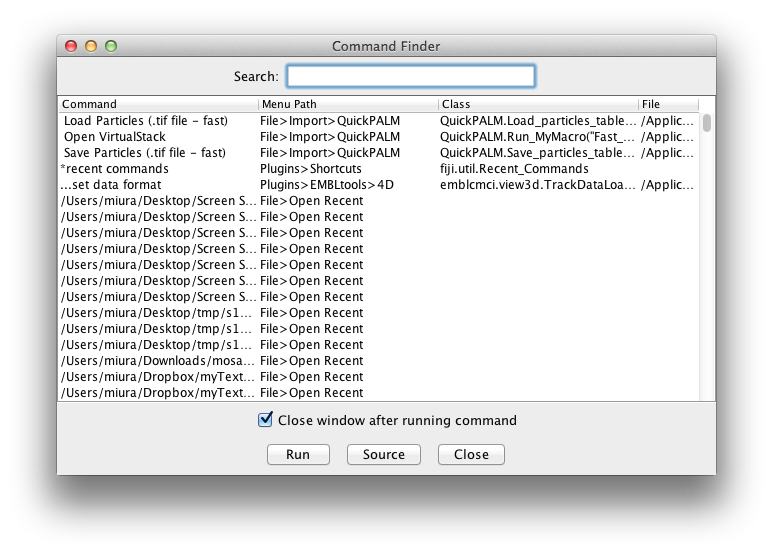
\includegraphics[width = 0.45\textwidth]{fig/commandFinder.png}}
\quad
\subfloat[Typing in some command name will filter the menu items and shows the hits.]{\label{fig:commandfinderConcat}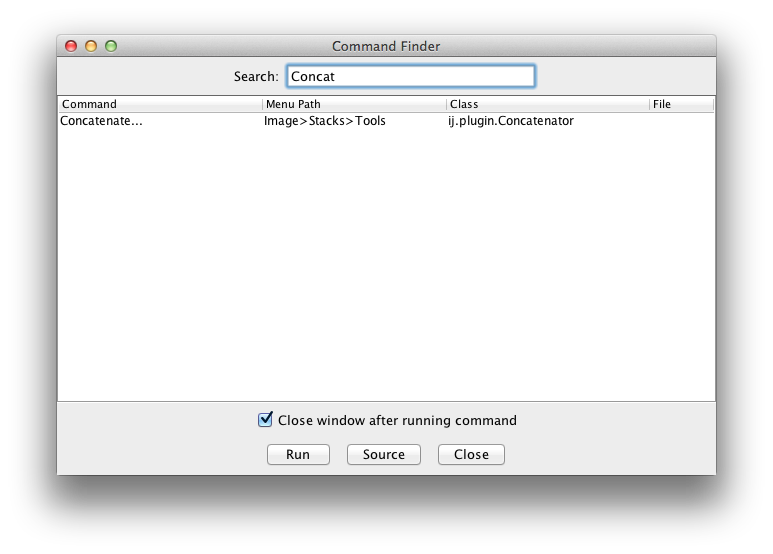
\includegraphics[width = 0.45\textwidth]{fig/commandFinderConcat.png}} 
\caption{Command Finder.}
\label{fig:commandfinder}
\end{figure}


\subsection{Visualization of Multidimensional Images}

We have an intrinsic limitation in displaying multidimensional images, but we still want to check data by our eyes. For this reason, ways to visualize multi-dimensional data have been developed. We go over some of those methods which are frequently used in this section. 

\subsubsection{Color Coding}

With multiple channels, we could have several different signal distributions per scene from different types of illuminations or from different types of proteins. One typical way to view such multiple channel image is to color code each channel \textit{e.g.} actin in red and Tubulin in green. We have already seen such images in the RGB section (\ref{subsec:rgb}). 

The color coding is not limited to the dimensions in Channels, but also for slices (Z) and time points (T). By assigning a color that depends on the slice number or time points, the depth information within a Z-stack or a time point information within a time lapse movie could be represented as a specific color rather than by the position of that slice or frame within image stack.


\begin{indentexercise}{1}
Open \ijmenu{[EMBL > Samples > TransportOfEndosomalVirus.tif ]}. Apply the color coding to this time-lapse movie \ijmenu{[Image > HyperStacks > Temporal-Color Code]}. In the dialog choose a color coding table from the drop-down list. Principle of the coding is same as the look-up table, and only the difference is that the color assignment is adjusted so that the color range of that table fits to the range of frames (Fig. \ref{fig:temporalColorcoding}). 


\begin{figure}[h!]
\centering
\subfloat[Original stack, first frame. This stack consists of 72 frames.]{\label{fig:TimeColorCodeOrg}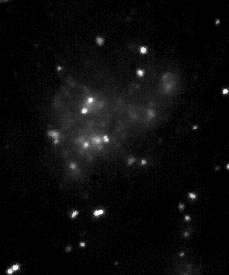
\includegraphics[width = 0.45\textwidth]{fig/TimeColorCodeOrg.png}}
\quad
\subfloat[Color coded stack.]{\label{fig:TimeColorCode}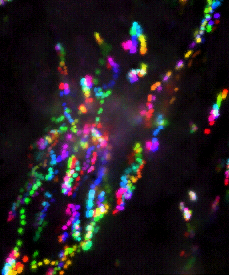
\includegraphics[width = 0.45\textwidth]{fig/TimeColorCode.png}} \\
\subfloat[Scale of the time color-coding. From frame 1 to 72, corresponding color is shown as a scale. ]{\label{fig:TimeColorCodeScale}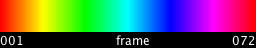
\includegraphics[width = 0.8\textwidth]{fig/TimeColorCodeScale.png}}
\caption{Temporal-Color Coding.}
\label{fig:temporalColorcoding}
\end{figure}

\end{indentexercise}

 

\subsubsection{Projection}

Projection is a way of decreasing an \textit{n}-dimensional image to an \textit{n-1}-dimensional image. For example, if we have a three dimensional XYZ stack, we could do a projection along Z-axis to squash the depth information and represent the data in 2D XY image. We lose the depth information but it helps us to see how the data looks like. The principle is like this: we could think of XYZ data as a cubic entity. This cube is gridded and composed of small cubic elements. If we have a Z-stack  with 512 pixels in both XY and with 10 slices in Z, we then have a 
cube composed of 512 x 512 x 10 =  2,621,440 small cubes. These small cubes are called ``voxels'', instead of ``pixels''. Now, if we take a single XY position, there are 10 voxels at this XY position (figure \ref{fig:projectionscheme}).
 
Imagine the column of 10 voxels: Each voxel has a given intensity, and we can compute statistics over these 10 values such as the mean, the minimum, the maximum, the standard deviation and so on. We can then represent this column by a single statistical value.  

\begin{figure}[h!]
\begin{center}
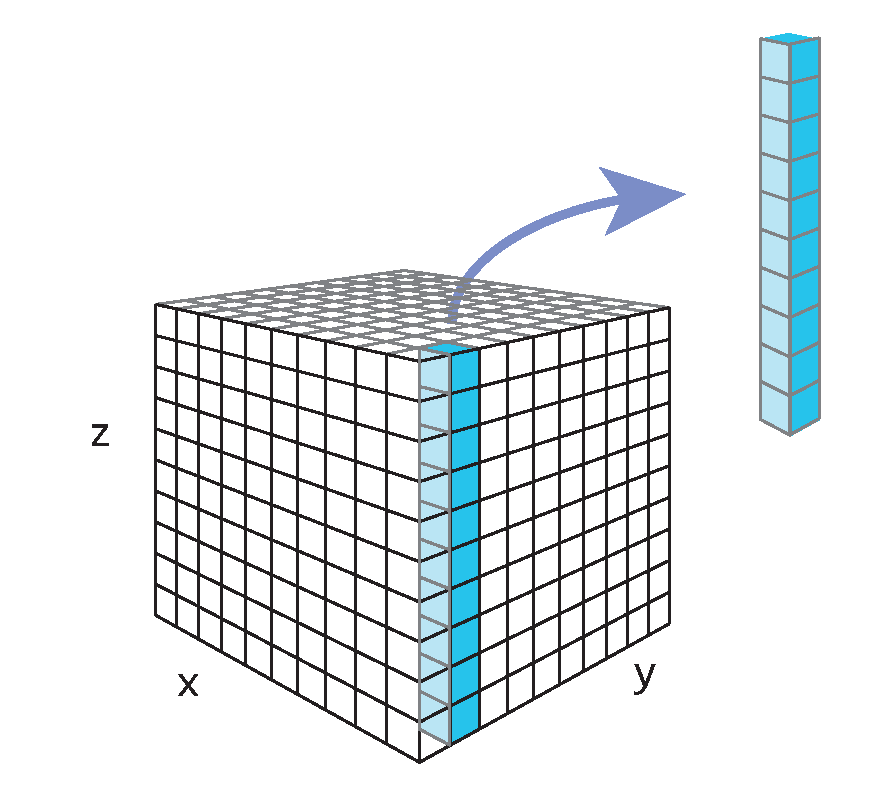
\includegraphics[scale=0.8]{fig/projection.pdf}
\caption{A three dimensional stack can be regarded as a gridded cube. The projection calculates various sorts of statistics for each two dimensional positions , which can be viewed as a stack of voxels, and store that value in the two dimensional image at the same position.}
\label{fig:projectionscheme}
\end{center}
\end{figure}

In this way, we can pick up a column of voxels from every XY positions, compute statistics and create a two dimensional image with each of its XY position filled with voxel column statistics. This two dimensional image is the result of the \textbf{projection} along Z-axis, or what we call ``Z-projection''. Projection could also be in other axes, not only along Z-axis. If we do a projection along X-axis, we would then have a projection of the data to YZ plane. Projecting aloing Y-axis will result in a projection to XZ plane (this relates to the orthogonal viewing, which we try in the next section).

\begin{indentexercise}{2}
Open image \textbf{mitosis\_anaphase\_3D.tif}.
Then do all types of projections you could choose in \ijmenu{[Image > Stack > Z
projection\ldots]}.\\
There are 
\begin{itemize}

    \item Average Intesnity
\item Max Intensity
\item Min Intensity
\item Sum of Slices
\item Standard Deviation
\item Median
\end{itemize}

\textbf{Question 1}: Which is the best method for knowing the shape of the chromosome?\\
\textbf{Question 2}: Discuss the difference of projection types and why there is such a difference.  
\end{indentexercise}

``Max Intensity'' projection is the most frequently used projection method in fluorescence microscopy images, as this method picks up bright signals. ``sum of slices'' method returns a 32bit image since results of addition could possibly exceed 8 bit or 16 bit range. 

Note 1: If your data is a 3D time series hyper stack, there will be a small check box in the projection dialog "All Time Points". If you check the box, projection will be done for each time point and the result will be a 2D time series of projections.

Note 2: The projection of a 2D time series can also be performed. Thought the command name is ``Z-Projection'', the principle of projection is identical regardless of the projection axis.  

\subsubsection{Orthogonal Views}

The projection is a convenient method for visualizing 3D stack on 2D plane, but if you want to preserve the original dimensions and still want to visualize data, one way is to use a classic 2D animation. This could be achieved easily with the scroll bar at the bottom of the each stack. But this has limitation: we could only move in the third dimension, Z or T. To scroll through X or Y, we use ``Orthognlal View''. 

You could view a stack in this mode by \ijmenu{[Image > Stack > Orthogonal View]}. Running this command will open two new windows at the right side and below the stack. These two new windows are showing YZ plane and XZ plane. Displayed position is indicated by yellow crosses. These yellow lines are movable by mouse dragging. 

\begin{figure}[h!]
 \centering
 \subfloat[XY]{\label{fig:OrthoViewXY}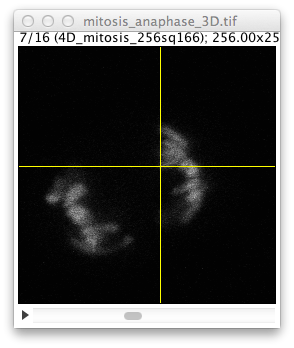
\includegraphics[height = 0.2\textheight]{fig/OrthoViewXY.png}} 
% \quad
 \subfloat[YZ]{\label{fig:OrthoViewYZ}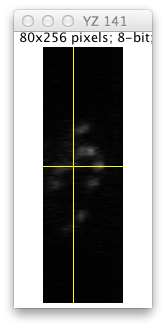
\includegraphics[height = 0.2\textheight]{fig/OrthoViewYZ.png}}
\\
 \subfloat[XZ]{\label{fig:OrthoViewXZ}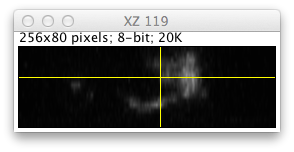
\includegraphics[height = 0.09\textheight]{fig/OrthoViewXZ.png}}
 \caption{Orthogonal views of a 3D stack.}
 \label{fig:orthogonalView}
\end{figure}

\begin{indentexercise}{3}
Open image \textbf{mitosis\_anaphase\_3D.tif}.
Run a command \ijmenu{[Image > Stack > Orthogonal View]}. Try scrolling through each axes: x, y and z. 
\end{indentexercise}

\subsubsection{3D viewer}

Instead of struggling to visualize 3D in 2D planes, we could also use the power of 3D graphics to visualize three dimensional image data. 3D viewer is a plugin written by Benne Schimidt. It uses Java OpenGL (JOGL) to render three dimensional data as click-and-rotatable object on your desktop. We could try to use the 3D viewer with the data we have been previously dealing with. 

\begin{indentexercise}{4}
Open image \textbf{mitosis\_anaphase\_3D.tif}.
Run a command \ijmenu{[Plugins > 3D Viewer]}. A parameter input dialog opens on top of 3Dviewer window. Change the following parameters:
\begin{itemize}
\item Image: Choose mitosis\_anaphase\_3D.tif.
\item Display as: Choose Surface.
\item Color: Could be any color. In the example shown in fig.\ref{fig:3DviewerSurface}, white was chosen. 
\item Threshold: Default value 50 should work OK, but you could also try changing it to greater or smaller values. This threshold value determines the surface. Pixel intensity greater than this value will be considered as object, else background. 
\item Resampling factor: default value (2) should be sufficient. If you change this value to 1, then it takes longer time for rendering. In case of our example image which is small, difference in the rendering time should be not really recognizable. 
\end{itemize}

After setting these values, clicking ``OK'' will render the image in the 3Dviewer window. Try to click and rotate the object. 

\begin{figure}[h!]
 \centering
 \subfloat[Parameter Input Dialog]{\label{fig:3DviewerParameters}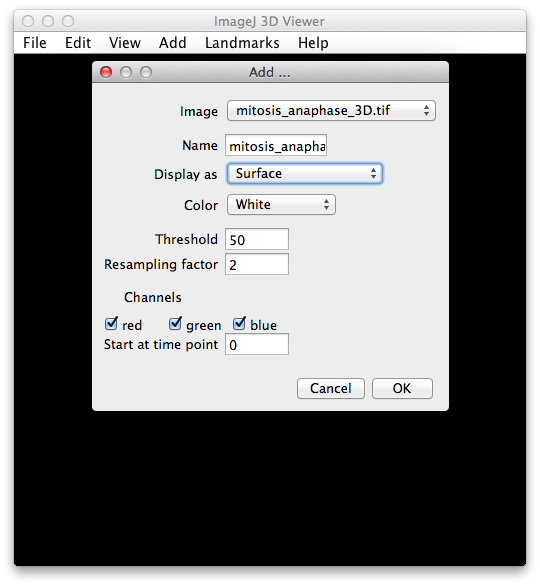
\includegraphics[width = 0.45\textwidth]{fig/3DviewerOptions.png}} 
 \quad
 \subfloat[Surface rendered 3D stack]{\label{fig:3DviewerSurface}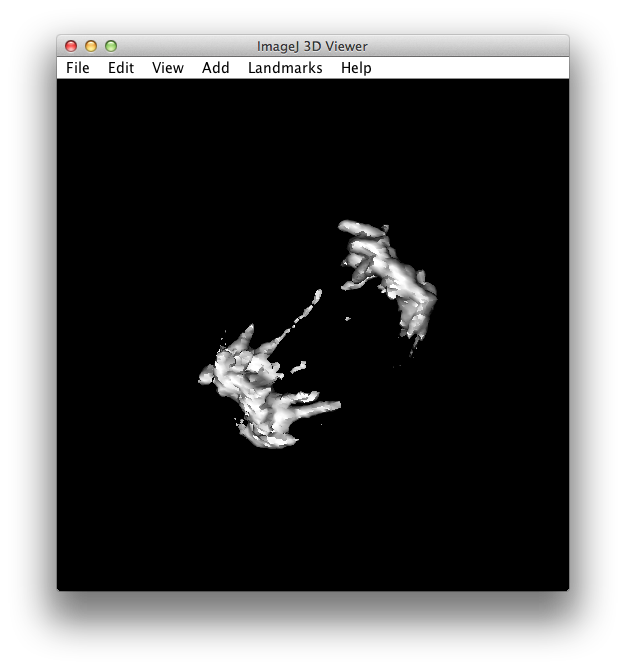
\includegraphics[width = 0.45\textwidth]{fig/3DviewerExample.png}}
 \caption{Surface rendering by 3DViewer.}
 \label{fig:3DviewerSurface}
\end{figure}
\end{indentexercise}

More advanced usages are available such as visualizing two channels or showing 3D time series as a time series of 3D graphics or saving movies. For such usages, consult the tutorial in the 3DViewer website (\url{http://3dviewer.neurofly.de/}).  

\subsection{Resampling images (Shrinking and Enlarging)}

When you want to check the details of images, zooming is the best way to focus on a specific region to observe details.  Zooming is done by the magnification tool (icon of
magnification glass) and this simply enlarges or shrinks the pixels.

Instead if you really need to increase the number of pixels per distance, we call such processing as ``Resampling'' and we will examine this a bit in this section. 

By the way, if we just want to have larger image by adding some margin, we call this ``resizing'', and the command for this resides in the menu tree: \ijmenu{[Image > Adjust > Canvas Size]}.

The resampling changes the original data. If we
have an image of size 10 pixels by 10 pixels and resample it to 200\%, the image
becomes 20 x 20.
If we resample it by 50\%, then the image becomes 5 x 5. The resampling is a simple task
that could be done by \ijmenu{[Image > Adjust > Size\ldots]}. This is a simple
operation but one must take care about how pixels will be produced while
enlarging and reduced while shrinking. If the enlarging is simply two times
larger, we could imagine that each pixel will be copied three times to produce a
block of four pixels to complete the task. The pixel values of the newly
inserted pixels will then be identical to the source pixel.

But what happens if we want to enlarge the image by 150 \%? To simplify the
situation, think about an image with 2 x 2 pixels. Then the resulting image
becomes 3 x 3. To understand the effect, do the following exercise.


\begin{indentexercise}{1}
Open the example image
4pixelimage\_sample.tif. The image is ultra small, so zoom it
up to the maximum (as much as you can, you must click on or
\textit{Ctrl - +}). You now see four pixels in the window.
Duplicate the image by \ijmenu{[Image > Duplicate]}.
Magnify again. "Select all" by
\ijmenu{[Edit > Selection > Select All]}.
Then \ijmenu{[Image > Adjust > Size\ldots]}.
In the dialog window, input the width 4 and height 4 (corresponds to
200\% enlargement). Tick "aspect
ratio" and
un-tick "Interpolation". Then click
OK. Check the pixel values in original image, and the enlarged image.
\end{indentexercise}

\begin{indentexercise}{2}
Do the similar resampling, but this time enlarge
the image by 150\%. Check the pixel values.
%double figure
\begin{figure}[htbp]
\centering
\subfloat[]{\label{fig:img28}
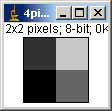
\includegraphics[width=3.951cm,height=3.916cm]{fig/CMCIBasicCourse201102-img28.jpg}
}
\subfloat[]{\label{fig:img29}
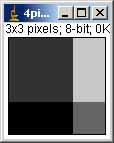
\includegraphics[width=4.022cm,height=5.045cm]{fig/CMCIBasicCourse201102-img29.jpg}
}
\caption{ Artifacts produced by resizing. (a) Four pixel image and (b) nine pixel image after
resizing. }
\label{fig:resizing}
\end{figure} 

\end{indentexercise}

The resampling in the exercise was without interpolation -- the check box
was OFF. Interpolation is similar to the one dimensional interpolation
we do with graphs. In case of images, the gradient is also two
dimensional so the situation is a bit more complex. There are various
methods for interpolating image. The interpolation method used in
ImageJ is the \textit{bilinear interpolation}. Briefly, the bilinear
interpolation algorithm samples pixel values in the surrounding of the
insertion point, and calculates the pixel value for that
position\footnote{\ For more details on bilinear interpolation, refer
to\\
http://www.cambridgeincolour.com/tutorials/image-interpolation.htm.}.
One must keep in mind that the result of enlarging or shrinking of
image depends on the interpolation method -- and scientific results
could be altered depending on the method you use. In a more general context, this problem is treated as ``sampling theory''. With this keyword, search more explanation in information theory textbooks and in the Internet. 

\clearpage
\subsection{ASSIGNMENTS }%%%%%%%%%%%%%%%%%%%%%%%

\textbf{\sffamily
Assignment 1-1-1: Digital image = matrix of numbers}

Edit a text image using any text editor. Be sure to insert space between
numbers as separator. Save the text file and open it as an image in
ImageJ by importing text image function. \ \ 

\textbf{\sffamily
Assignments 1-1-2: bit depth}
\begin{enumerate}
\item How many gray scale steps does a 12-bit image have?\\
\item Describe in text how a 1-bit image looks like.
\end{enumerate}

\textbf{\sffamily
Assignment 1-1-3: bit depth conversion}

Use m51.tif (16-bit!) sample image to draw a plot profile, as we did in
the course. In the profile plot window, a
"list" button is at the left-bottom corner.
Click the button. You will then see a new window containing a column of
numbers. These numbers can be copy \& pasted to spread sheet software
such as LibreOffice Calc or MS Excel. Overlay the three curves in a graph,
and observe the differences. 

\textbf{\sffamily
Assignments 1-1-4: Simple math on Images}
\begin{enumerate}
\item Try subtracting certain values from the image you created in
the Assignment 1-1-1 and check that the values cannot be less than 0. 
\item Prepare an 8-bit image with pixel value 200. Divide the
image by 3, and check the result. 

\item Prepare a 16-bit image. In the \ijmenu{[File > New > 
Image\ldots]} dialog, select 16-bit from the
"type" drop-down menu. Try adding
certain value to check the maximum pixel value. 

\item Discuss why measurement of fluorescence intensity using
digital image is invalid when some pixels are saturated. 
\end{enumerate}

\textbf{\sffamily
Assignments 1-1-5: LUT}

Open "Cell\_Colony.tif". Use LUT edit function and design your own LUT to highlight the black dots in
Green and the background in Black. "LUT editor" can be activated by \ijmenu{[Images > Color > Edit LUT\ldots]}. Instruction for the LUT editor is at\\
\url{http://rsb.info.nih.gov/ij/plugins/lut-editor.html} \\
You might be able to manage using it without reading the web instruction; just try!). LUT (.lut file) could also be edited using Excel. 

\textbf{\sffamily
Assignments 1-1-6: File size and image bit depth, image size}

If there is an image with width = 100 pixels and height = 200 pixels,
what would be the expected size of the image file in bytes? 1 byte =
8-bit.

Create a new image with the dimension as above, and save the image in
"bitmap (.bmp)" format and check the file
size. Is it same as you expected, or different? Save the same image in
text file format and check the file size again.

\textbf{\sffamily
Assignment 1-1-7 Resizing}

\begin{enumerate}
\item Enlarge the sample image 4pixelimage\_sample.tif by
150\% while the "Interpolation"
check box in the size adjustment window is ON. Study the pixel values
before and after the enlargement. What happened? Describe the result.

\item Change "canvas size" by \ijmenu{[Image > Adjust > Canvas Size]} for any image. What"s the
difference to "Resize"?
\end{enumerate}


